\subsubsection{H-Brücke}
\label{subsubsec:H-Brücke}

Das Bindeglied zwischen Kraft (Motor) und Steuersignalen wird von der H-Brücke gebildet. Durch Laden-/Entladen der MOSFET-Gates wird eine Spannung an einer Spule angelegt oder weggenommen. Wie sich das Ein- und Ausschalten der einzelnen Phasenbrücken auf den Motor auswirkt, wird zu einem späteren Zeitpunkt erklärt\todo{Referenzierung auf mögliches Kapitel FOC-Steuerung mit BLDC-Motor / Reglerauslegung}.

\paragraph{Schaltungsaufbau}\mbox{}

Für den Aufbau und die Dimensionierung wurde das Referenzschema des Evaluationsboard verwendet, mit dem getestet wurde (Trinamic UPS 10A70V). Es ist aufgezeigt im Anhang Kapitel \ref{Appendix:H_Bruecke} Abbildung \ref{fig:Schema_H_Bruecke_und_BLDC_Ref}. Die Dimensionierung der Shunts wird in Kapitel \ref{subsubsec:Gate-Treiber} abgehandelt.

Der Schltungsaufbau ergibt sich durch den dreiphasigen Aufbau des BLDCs. Es werden so drei Stränge gebildet, woran jeweils eine Spule verbunden wird. Der Energiefluss führt dabei über einen Strommesswiderstand. Die Eingänge der H-Brücke werden zusätlich mit Stütz- und Filterkondensatoren bestückt, um eine saubere Netzspannung zu gewährleisten.

\begin{figure}[h!]
	\centering
	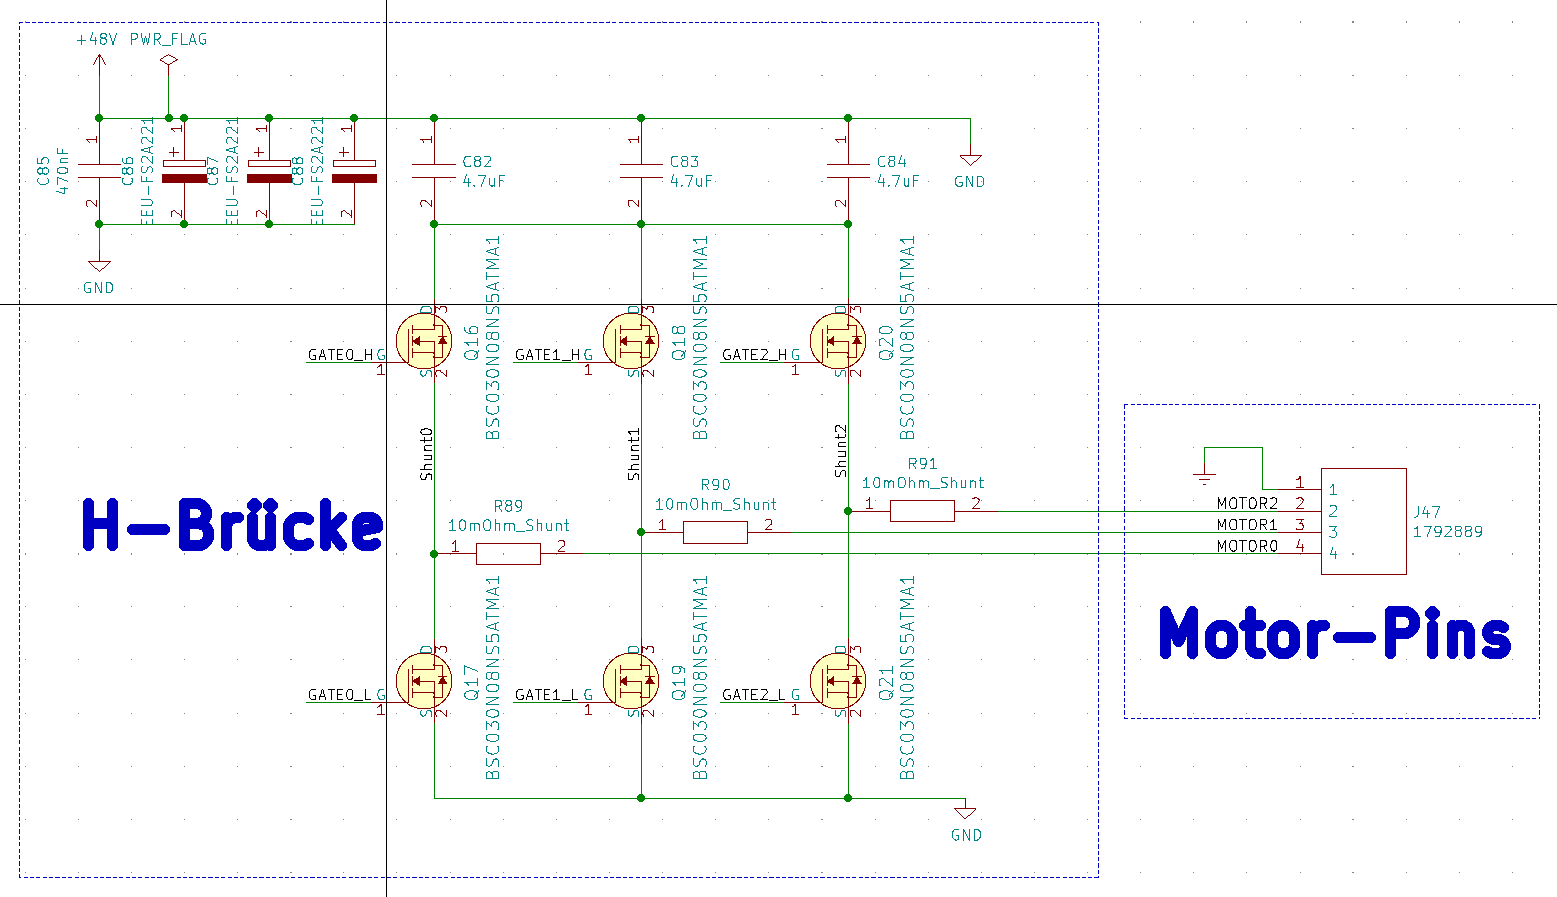
\includegraphics[width=0.7\textwidth]{graphics/Schema_H_Bruecke_und_BLDC}
	\caption{H-Brücke.}
	\label{fig:Schema_H_Bruecke_und_BLDC}
\end{figure}

\newpage

\paragraph{Funktionsbeschrieb}\mbox{}

Wie erwähnt werden die Eingänge gefiltert. Dies geschieht mit den Kondensatoren C85-C88, um die Eingangsspannung konstant zu halten und hochfrequente nicht ins Netz gespiesen werden.
Bei C86-C88 handelt sich um Low-ESR Stützkondensatoren, jeweils ein Kondensator pro Phase.
Sie befinden sich nahe am Spannungseingang und der H-Brücke.

Die Kondensatoren C82-C84 sind Kondensatoren, welche direkt zwischen Ein- und Ausgang eines H-Brücken-Strangs platziert wurden.
Sie dienen auch zu Filterzwecken.

Die MOSFETS Q16-Q21 bilden die eigentliche H-Brücke. Sie Schalten den Leistungsfluss gemäss den Ansteuersignalen. Sie können 100A Nennstrom schalten und 100V standhalten. Die Gate-Source-Spannung beträgt $\pm$20V.